姿态控制器获取到制导控制器计算得到的期望姿态数据组之后, 按照ALTCTL(RC)和OFFBOARD两种控制方式进行PID控制处理, 如图\ref{fig:atti}所示. 
\par OFFBOARD模式下, 将计算得到的欧拉姿态设定值转化为四元数, 以及根据自己欲控制的量为type$\_$\\mask进行赋值, 完成姿态的封装, 发布给PX4; 
RC模式下, 会根据当前无人机的欧拉姿态与期望欧拉姿态计算一个ERROR, 根据ERROR, 进行PID控制计算, 得到四个RC通道的值(roll, pitch, yaw, throttle), 发布给PX4. 
\begin{figure}[htbp]
    \centering
    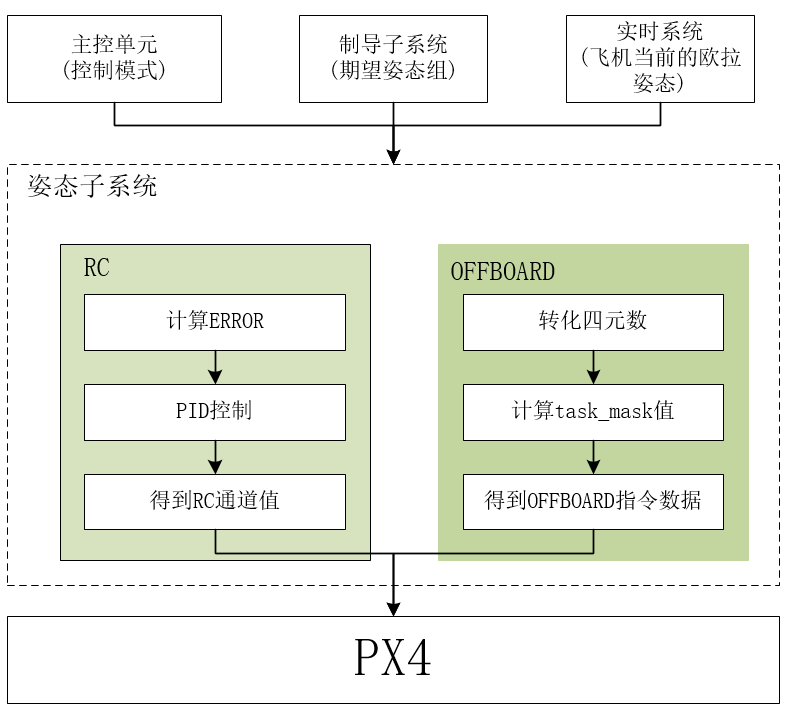
\includegraphics[width=0.8\textwidth]{pictures/attitudeCtrl.png}
    \caption{attitude controller}
    \label{fig:atti}
\end{figure}